\documentclass[tikz]{standalone}
\usepackage{tikz}
\usetikzlibrary{shapes,calc,arrows,through,intersections,angles}
\usepackage{xcolor}

\begin{document}

%----Proper document------------------------------------------------------------

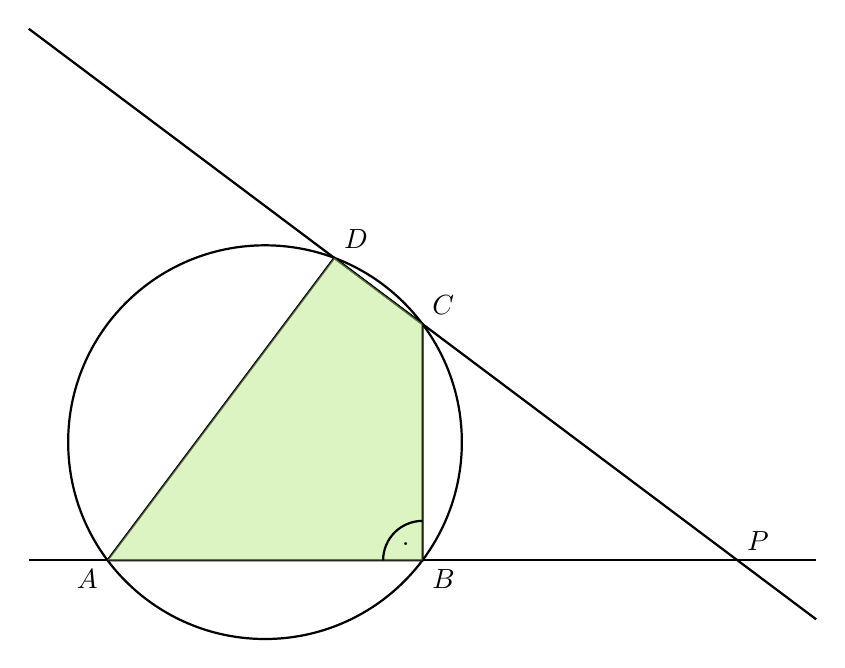
\begin{tikzpicture}[scale=0.5]

\definecolor{limegreen}{RGB}{184,233,134}

\coordinate (A) at (0,0);
\coordinate (B) at (8,0);
\coordinate (C) at (8,6);
\coordinate (D) at (144/25,192/25);
\coordinate (P) at (16,0);

\node at (A) [below left] {$A$};
\node at (B) [below right] {$B$};
\node at (C) [above right] {$C$};
\node at (D) [above right] {$D$};
\node at (P) [above right] {$P$};

\draw [thick] (-2,0) -- (18,0);
\draw [thick] (-2,27/2) -- (18,-3/2);
\draw [thick] (4,3) circle [radius=5];

\draw [thick] (A) -- (B) -- (C) -- (D) -- (A);

\fill[fill=limegreen,opacity=0.5] (A) -- (B) -- (C) -- (D) -- cycle;

\draw pic [draw,black,thick,pic text=.] {angle = C--B--A};

\end{tikzpicture}

%-------------------------------------------------------------------------------

\end{document}
